\renewcommand{\this}{PCA}

\chapter{Principle Component Analysis (PCA)}
	\section{Matrix factorization as a tool}
		The core concept of principle component analysis is making use of matrix factorization techniques. These techniques, as the name implies, decompose a matrix of interest $X \in \Real^{m \times n}$ into several matrices such that their product equals $X$. For example, an approximation of the data matrix $X$ could be given by the product of $A \in \Real^{m \times k}$ and $B \in \Real^{k \times n}$:\\
		\begin{figure}[h!]
			\centering	
			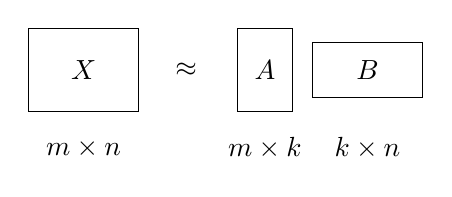
\begin{tikzpicture}
			\draw (0,0) node[shape=rectangle, draw=black, minimum width = 40, minimum height = 30](x){$X$};
			\draw node[below of = x] (times) {$m \times n$};
			
			\draw node[right of = x, xshift = 2ex] (apr){$\approx$};
			
			\draw node[right of = apr, shape=rectangle, draw=black, minimum width = 20, minimum height = 30](A){$A$};
			\draw node[below of = A] (times) {$m \times k$};
			
			\draw node[right of = A, shape=rectangle, draw=black, minimum width = 40, minimum height = 20, xshift = 2ex](B){$B$};
			\draw node[below of = B] (times) {$k \times n$};
			\end{tikzpicture}
			\label{approx}
			\caption{Example of factorization.}
		\end{figure}\\
		A whole range of practical problems can be written as a matrix factorization problems. Often we can gain a lot of insights based on decompositions.
\\\\
In the previous example, the matrix $X$ was a $m \times n$ matrix. 
It was decomposed into $m \times k$ and $k \times n$ matrices. 
Naturally, $A$ and $B$ share a dimension such that their product
is defined. In matrix factorization problems this is almost always
the case. This $k$ can be chosen differently based on the problem 
you are dealing with. For example, if one wants to decompose a 
matrix without losing any information at all, one chooses 
$k = \min(m, n)$. It is not always desirable to decompose a 
given matrix, without losing information. In most cases one is
interested in smaller $k$ values. Be it for reducing dimension, 
easier understanding of the decomposition, memory and time 
considerations.

\section{Frobenius norm as a closeness metric}
When using a $k$ value smaller than $\min(m, n)$, we lose 
information when decomposing matrix $X \Real^{m\times n}$.
The decomposition then becomes an approximation $X \approx AB$
As we don't want to lose too much information, we need a 
measure of how \textit{close} two matrices are. 
One of the ways we can measure this is using the frobenius norm:
\begin{equation}
	d(A, B) = \norm{A - B}_F
\end{equation}
Assume again, we wish to find a matrix decomposition of $X$ where 
$k$ is small, so we lose information, the decomposition is
an approximation. We would then measure how good this approximation
is using the frobenius norm:
\begin{equation}
	d(X,AB) = \norm{X - AB}_F
\end{equation}
Transforming this into a minimization objective:
\begin{equation}
	\underset{A,B}{\min}\norm{X - AB}_F
\end{equation}
	
\section{PCA as dimension reduction}
PCA is primarily a technique to \textit{reduce the dimension} of 
a given data set $X$. Assume there are $n$ data points
of dimension $m$, i.e.
$\mathcal{X} = \{x_i| x_i \in \Real^m, i \in \{1\dots n\}\}$.
Conveniently, this can be encapsulated as a matrix 
$X \in \Real^{n \times n}$. We can then decompose the 
matrix as before into $A \in \Real^{m \times k}$ and 
$B \in \Real^{k \times n}$. Assume now that $k$ is 
significantly smaller $\min(m,n)$. Instead of having 
$\mathcal{O}(mn)$ values we now only have $\mathcal{O}(k(m+n))$
values. For a large $m$ this is significant. The above
was an example of dimension reduction. PCA is an example of 
such a dimension reduction techniques. Even more, it is 
one of the most used techniques out there for reducing dimension.

\begin{exmp}
As an example we could look at an approximation of a face using PCA.
\begin{figure}[h!]
	\centering
	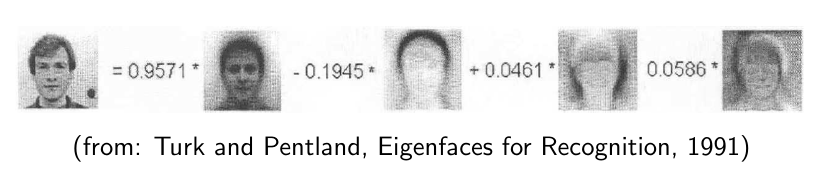
\includegraphics[scale=0.5]{\figDir/face_ex.PNG}
\end{figure}\\
The dimension of the original data points is the 
exact amount of pixels in the image. Perhaps the amount
of pixels is unmanageable. In this example, the faces were
are reconstructed using $k=4$ images. Thus, instead of 
considering each data point as a collection of pixels,
we reduced the dimension of the data by considering each data 
point as a combination of $4$ base images. We have reduced 
the dimension of the data to $4$. Of course, in order 
to re-construct the original images, the $4$ base images 
are required.
\end{exmp}

\section{Reducing data to a single value}
In order to see what PCA does exactly, we will first
consider what would happen if we reduced the $m$ dimensional
data to a single value. Hopefully, this value will contain 
the most information as possible. In essence we are looking 
at what would happen as $k = 1$. In order to reduce each data 
point to a single value, many approaches exist. Take for example
the approach where we simply take the euclidean norm of each point.
In this case, we capture some information but we lose a lot
of information. To see why consider $(0, 1)$ and $(1, 0)$.
They are perpendicular, yet $\norm{(0,1)} = \norm{(1,0)}$.
\\\\
There are better ways. We could for instance reduce the points
by projecting them onto a single line. This is actually the first
and only step in PCA. By iterating this exact step we obtain
the PCA decomposition. We start by projecting onto a single line.

\subsection{Lines, minimizing distance and projection}
Before we project onto it, we need to define exactly what 
is meant with a line in the $\Real^m$ space.
One way to define a line is as follows:

\begin{defn}
\begin{equation}
a + \Real b \equiv \{x \in \Real^m | 
\exists z \in \Real \text{ s.t. } x = a + zb\}
\end{equation}
Here, $a$ is sometimes referred to as the offset or intercept
and $b$ is sometimes referred to as the direction of the line.
\end{defn}
			
\begin{figure}[h!]
	\centering
	\begin{tikzpicture}[scale = 0.5]
	\draw[->] (-1,0) -- (5,0);
	\draw[->] (0,-1) -- (0,5);
	\draw[->, red, thick] (0,0) -- node[xshift = 1.5ex](lab){a}(1,2);
	\draw[->, blue, thick] (1,2) -- node[xshift = 1.5ex](lab){b}(2,1);
	\draw[blue, dashed] (-1,4) -- node[xshift = 1.5ex](lab){b}(4,-1);
	\end{tikzpicture}
	\label{fig:line}
	\caption{Visual of a line}
\end{figure}

Figure \ref{fig:line} gives an intuitive idea of 
what a line in $\Real^2$ looks like. Often we want the 
direction to have unit length, that is: $\norm{b}_2 = 1$. 
Say we want to reduce data to a single line, we need a 
specific objective (i.e. a specific function that defines 
how good the line/reduction to the line is). We can achieve
this by using e.g. the squared euclidean distance. 
Intuitively you would think that your data point should be 
quite close to the chosen point on the line. This is exactly 
what the euclidean distance defines, how close our reduced 
point is to the actual data point. We define how \textit{good}
the reduction is to the single line (using euclidean 
distance as measure) as follows:

			\begin{equation}
				\underset{z\in\Real}{\text{arg min}} \norm{a + bz - x}^2
			\end{equation}
			Figure \ref{fig:sq} shows an intuitive picture of the \textbf{non squared} euclidean distance.
			\begin{figure}[h!]
				\centering
				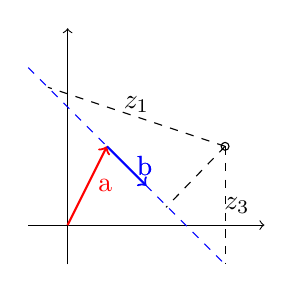
\begin{tikzpicture}[scale = 0.5]
					\draw[->] (-1,0) -- (5,0);
					\draw[->] (0,-1) -- (0,5);
					
					\draw (4,2) circle (0.1cm);
					
					\draw[->, red, thick] (0,0) -- node[xshift = 1.5ex](lab){a}(1,2);
					\draw[->, blue, thick] (1,2) -- node[xshift = 1.5ex](lab){b}(2,1);
					\draw[blue, dashed] (-1,4) -- node[xshift = 1.5ex](lab){b}(4,-1);
					
					\draw[dashed] (4,2) -- (2.5,0.45);
					\draw[dashed] (4,2) -- node[yshift = 1ex] {$z_1$} (-0.5,3.5);
					\draw[dashed] (4,2) -- node[xshift = 1ex] {$z_3$}(4,-1);
				\end{tikzpicture}
				\caption{Visual of distance to a line for varying $z$ values}
				\label{fig:sq}
			\end{figure}\\
			It is clear to see that using this criteria that we reach the minimal value of $\norm{\cdot}$ when $z$ is chosen such that we project orthogonally onto the line as in figure \ref{fig:sq}. Mathematically we can derive this as where the (convex) loss is minimal:
			\begin{equation}
			\label{eq:sol_z}
				\begin{split}
					\der{z}\norm{a + bz - x}^2 &= 2(a +bz - x)^T b = 0 \\
					  &=(a-x)^T b + \underbrace{b^Tb }_{\norm{b}^2 = 1}z = 0\\
					z &=-(a-x)^Tb
				\end{split}
			\end{equation}
			This comfirms our belief of the orthogonal projection, since we are projecting onto the $b$ direction. To understand exactely what's happening we can see in figure \ref{fig:proj}, the green arrow ($x-a$) is being projected onto $b$ to find the optimal $z$.
			\pagebreak
			
			\begin{figure}[h!]
				\centering
				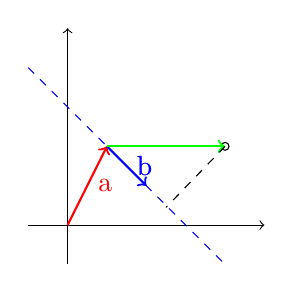
\begin{tikzpicture}[scale = 0.5]
					\coordinate[](origin) at (0,0) ;
					\coordinate[](a) at (1,2) ;
					\coordinate[](b) at (2,1) ;
					\coordinate[](x) at (4,2) ;
					
					\draw[->] (-1,0) -- (5,0);
					\draw[->] (0,-1) -- (0,5);
					
					\draw (x) circle (0.1cm);
					
					\draw[->, red, thick] (origin) -- node[xshift = 1.5ex](lab){a}(a);
					\draw[->, blue, thick] (a) -- node[xshift = 1.5ex](lab){b}(b);
					\draw[blue, dashed] (-1,4) -- node[xshift = 1.5ex](lab){b}(4,-1);
					
					\draw[thick, green, ->] (a)--(x);
					\draw[dashed] (4,2) -- (2.5,0.45);
				\end{tikzpicture}
				\caption{Visual of optimal $z$ value as a projection of $(x-a)$ onto the direction.}
				\label{fig:proj}
			\end{figure}
			Now that we found the $z$ value that minimizes the loss (the projection onto the direction) let's look at what this means visually when we plug in the optimal $z$ into $a + bz$:
			\begin{figure}[h!]
				\centering
				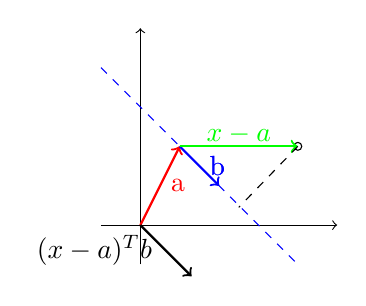
\begin{tikzpicture}[scale = 0.5]
					\coordinate[](origin) at (0,0) ;
					\coordinate[](a) at (1,2) ;
					\coordinate[](b) at (2,1) ;
					\coordinate[](x) at (4,2) ;
					
					\draw[->] (-1,0) -- (5,0);
					\draw[->] (0,-1) -- (0,5);
					
					\draw (x) circle (0.1cm);
					
					\draw[->, red, thick] (origin) -- node[xshift = 1.5ex](lab){a}(a);
					\draw[->, blue, thick] (a) -- node[xshift = 1.5ex](lab){b}(b);
					\draw[blue, dashed] (-1,4) -- node[xshift = 1.5ex](lab){b}(4,-1);
					
					\draw[thick, green, ->] (a)--node[yshift = 1ex]{$x-a$}(x);
					\draw[dashed] (4,2) -- (2.5,0.45);
					\draw[black, ->, thick] (origin) --node[xshift = -6ex] {$(x-a)^Tb$} (1.3,-1.3);
				\end{tikzpicture}
				$\Rightarrow$
				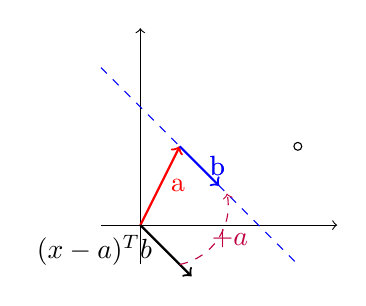
\begin{tikzpicture}[scale = 0.5]
					\coordinate[](origin) at (0,0) ;
					\coordinate[](a) at (1,2) ;
					\coordinate[](b) at (2,1) ;
					\coordinate[](x) at (4,2) ;
					
					\draw[->] (-1,0) -- (5,0);
					\draw[->] (0,-1) -- (0,5);
					
					\draw (x) circle (0.1cm);
					
					\draw[->, red, thick] (origin) -- node[xshift = 1.5ex](lab){a}(a);
					\draw[->, blue, thick] (a) -- node[xshift = 1.5ex](lab){b}(b);
					\draw[blue, dashed] (-1,4) -- node[xshift = 1.5ex](lab){b}(4,-1);
					\draw[black, ->, thick] (origin) --node[xshift = -6ex] {$(x-a)^Tb$} (1.3,-1.3);
					
					\draw[dashed, ->, bend right = 45, purple](1,-1)to node[xshift = 1ex]{$+a$}(2.2,0.8);
				\end{tikzpicture}
				\caption{Visual of optimal $z$ value plugged back in to find the optimal point again.}
				\label{fig:recon}
			\end{figure}\\
			Mathematically of course this means nothing else than the following:
			We can clearly see 4 steps in this process of finding the optimal value and "plugging it back in":
			\begin{enumerate}
				\item shift $x$ towords the bias $a$ by taking the difference: $x-a$
				\item projection onto the $b$ direction: $(x-a)^Tb$
				\item Multiply in the $b$ direction: $(x-a)^Tbb$
				\item Shifting back to the bias: $(x-a)^Tbb + a$
			\end{enumerate}
			
			\subsection{Finding optimal line through first order optimality conditions}
			So now we could also wonder the following: \textit{How do we choose the $a$ and $b$ such that we minimize some loss function?}. Consider again $n$ data points $\{x_1,...,x_n\}$ where $x_i \in \Real^m$. For example, how do we find the optimal line considering the euclidean squared loss:
			\begin{equation}
				L(a,b) = \frac{1}{n}\sum_{i=1}^{n}\norm{a + bz_i - x_i}
			\end{equation}
			Minimizing over $a,b,z_i$ and using previous results of equation (\ref{eq:sol_z}) we find:
			
			\begin{equation}
			\label{eq:loss}
				\begin{split}
					\underset{a,b,z_i}{argmin}\frac{1}{n}\sum_{i=1}^{n}\norm{a + bz_i - x_i}^2 &= \underset{a,b}{argmin}\frac{1}{n}\sum_{i=1}^{n}\norm{a + b(x_i - a)^Tb - x_i}^2\\
					&= \underset{a,b}{argmin}\frac{1}{n}\sum_{i=1}^{n}\norm{bb^T(x_i - a) + (a - x_i)}^2 \\
					&= \underset{a,b}{argmin}\frac{1}{n}\sum_{i=1}^{n}\norm{(bb^T - \ID)(x_i - a)}^2 \\
				\end{split}
			\end{equation}
			Note that the $\norm{\cdot}$ operation is an even function so \ref{eq:loss} can be written equivalently as (we can change the sign in the brackets $\norm{-a} = \norm{a}$):
			\begin{equation}
				\underset{a,b}{argmin}\frac{1}{n}\sum_{i=1}^{n}\norm{(\ID - bb^T)(x_i - a)}^2 \\
			\end{equation}
			Now what exactly does this equation mean? If we look at a general vector $v$:
			
			\begin{figure}[h!]
				\centering
				\begin{tabular}{c|c}
					$(\ID - bb^t)v = v - b(b^Tv)$
					&
					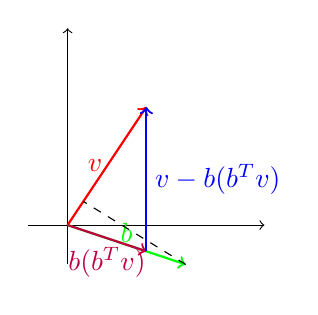
\begin{tikzpicture}[scale = 0.5]
					\coordinate[](origin) at (0,0) ;
					\coordinate[](v) at (2,3) ;
					\coordinate[](b) at (3,-1) ;
					
					\draw[->] (-1,0) -- (5,0);
					\draw[->] (0,-1) -- (0,5);
					
					\draw[->, thick, red] (origin)--node[xshift=-1ex]{$v$}(v);
					\draw[->, thick, green] (origin)-- node[yshift=1ex]{$b$}(b);
					\draw[->, thick, purple] (origin) --node[yshift=-2ex]{$b(b^Tv)$}(2,-0.666666666);
					\draw[->, thick, blue](2,-0.6666666666) --node[xshift = 6ex]{$v-b(b^Tv)$} (v);
					
					\draw[dashed] (b)--(0.4,0.6);
					\end{tikzpicture}
				\end{tabular}
				\caption{Visualisation of $(\ID - bb^T)v$}
			\end{figure}
			Another nice thing about $(\ID - bb^T)$ is that it is idempotent. A matrix $A$ is idempotent when $A^n = A$. We can show that this is clearly the case:
			\begin{equation}
				\label{eq:idempot}
				\begin{split}
					(\ID -bb^T)(\ID - bb^t) &= \ID\ID - 2bb^T + b\underbrace{b^Tb}_{bb^T = \norm{b}}b^T\\
					&= \ID - bb^T\\
				\end{split}
			\end{equation}\\
			\subsection{Optimal value for $a$}
			Now let's get back to finding the optimal line for the given data. The first order optimality condition (i.e. setting gradient w.r.t. $a$ to 0 and finding extremum value) of (\ref{eq:loss}) can be found as follows:
			\begin{equation}
				\label{eq:grad_Lin_loss_1}
				\begin{split}
					\nabla_a L(a,b) = \frac{-2}{n}(\ID - bb^T)^T(\ID - bb^T)\sum_{i=1}^{n}(x_i - a) &= 0
				\end{split}
			\end{equation}
			We now know that since $(\ID - bb^T)$ is clearly symmetric ($A^T = A$) and we know that the matrix is idempotent from (\ref{eq:idempot}), thus we can write (\ref{eq:grad_Lin_loss_1}) follows:
			\begin{equation}
				\label{eq:grad_Lin_loss_2}
				\begin{split}					
					\nabla_a L(a,b) = (\ID - bb^T)\sum_{i=1}^{n}(x_i - a) &= 0\\
					(\ID - bb^T)\sum_{i=1}^{n}(x_i) &= (\ID - bb^T)\sum_{i=1}^{n}(a)\\
					(\ID - bb^T)\frac{1}{n}\sum_{i=1}^{n}(x_i) &= (\ID - bb^T)a\\
				\end{split}
			\end{equation}
			From (\ref{eq:grad_Lin_loss_2}) we can see that the optimality condition is met when $a = \frac{1}{n}\sum_{i=1}^{n}x_i$. This means that the optimal line will always pass through the average of all the data points. Figure \ref{fig:avg} shows this visually:\\
			\begin{figure}[h!]
				\centering				
				\begin{tikzpicture}[scale=0.8]
				\coordinate[](origin) at (0,0) ;
				\coordinate[](x1) at (4,3) ;
				\coordinate[](x2) at (1,2.5) ;
				\coordinate[](x3) at (2,0.5);
				\coordinate[blue](av) at (2.3333333, 2);
				
				\draw (x1) circle (0.1);
				\draw (x2) circle (0.1);
				\draw (x3) circle (0.1);
				\draw[blue, thick, fill = blue] (av) circle (0.05) node[xshift = 2ex]{$\bar{x}$};
				
				\draw[dashed, red] (origin) -- (4.666,4) node[]{$l_1$};
				\draw[dashed, red] (-1,2) -- (5, 2) node[]{$l_2$};
				\draw[dashed, red] (0,4.3333) -- (5,-0.66666) node[]{$l_3$};
				
				\draw[dotted] (av)--(x1) node[xshift = 2ex]{$x_1$};
				\draw[dotted] (av)--(x2) node[xshift = -2ex]{$x_2$};
				\draw[dotted] (av)--(x3) node[xshift = -2ex]{$x_3$};
				
				\draw[->] (-1,0) -- (5,0);
				\draw[->] (0,-1) -- (0,5);
				\end{tikzpicture}
				\caption{Visualisation of lines going through average of data points $x_i$.}
				\label{fig:avg}
			\end{figure}\\
			The above figure shows us visually something quite interesting, since we know that the optimal line passes through the average $\bar{x}$ we could try to make the origin itself the average. We could achive this by substracting the average from every data point as in figure \ref{fig:subavg} below. This step is very often done as a preprocessing step. It makes derivations easier analytically. When "data is centered", this simply means that the emperical mean $\frac{1}{n}\sum_{i=1}^{n}x_i$ has already been substracted and that the new mean is the origin.
			
			\begin{figure}[h!]
				\centering				
				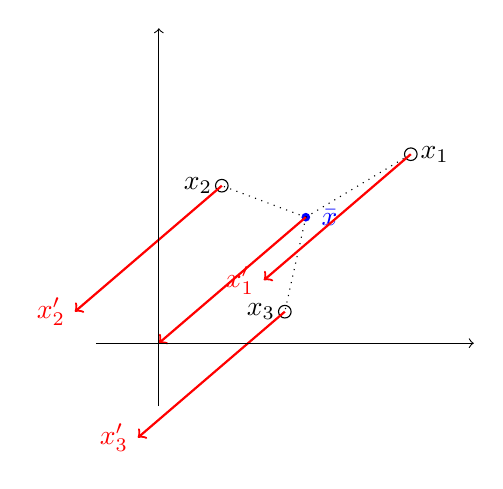
\begin{tikzpicture}[scale=0.8]
				\coordinate[](origin) at (0,0) ;
				\coordinate[](x1) at (4,3) ;
				\coordinate[](x2) at (1,2.5) ;
				\coordinate[](x3) at (2,0.5);
				\coordinate[blue](av) at (2.3333333, 2);
				
				\draw (x1) circle (0.1);
				\draw (x2) circle (0.1);
				\draw (x3) circle (0.1);
				\draw[blue, thick, fill = blue] (av) circle (0.05) node[xshift = 2ex]{$\bar{x}$};
				
				\draw[dotted] (av)--(x1) node[xshift = 2ex]{$x_1$};
				\draw[dotted] (av)--(x2) node[xshift = -2ex]{$x_2$};
				\draw[dotted] (av)--(x3) node[xshift = -2ex]{$x_3$};
				
				\draw[thick, red, ->] (av) -- (origin);
				\draw[thick, red, ->] (x1) -- ++(-2.33333,-2)node[xshift = -2ex]{$x_1'$};
				\draw[thick, red, ->] (x2) -- ++(-2.33333,-2)node[xshift = -2ex]{$x_2'$};
				\draw[thick, red, ->] (x3) -- ++(-2.33333,-2)node[xshift = -2ex]{$x_3'$};
								
				\draw[->] (-1,0) -- (5,0);
				\draw[->] (0,-1) -- (0,5);
				\end{tikzpicture}
				\caption{Visualisation of substracting mean of points from $x_i$.}
				\label{fig:subavg}
			\end{figure}
			\pagebreak
			\subsection{Optimal value for $b$ as principal eigenvectors}
			As figure \ref{fig:avg} suggests, this of course leaves the question of \textit{How do we choose the direction of the optimal line?} Now we assume that the data is centered, this means that $a$ in $a+bz$ is assumed to be $0$. If we then look at the euclidean loss function as in (\ref{eq:loss}), but assume no offset we obtain:
			\begin{equation}
				\begin{split}
					b&\in\underset{b}{argmin}\frac{1}{n}\sum_{i=1}^{n}\norm{x_i^Tbb - x_i}^2 \\
					b&\in\underset{b}{argmin}\frac{1}{n}\sum_{i=1}^{n}\norm{x_i^Tbb}^2 +\sum_{i=1}^{n} \norm{x_i}^2 - 2\sum_{i=1}^{n} (x_i^Tbb)^Tx_i \\
				\end{split}		
				\label{eq:loss_decomposed}		
			\end{equation}
			If we look at $\norm{x_i^Tbb}^2 = (x_i^Tbb)^Tx_i^Tbb = (x_i^Tb)\underbrace{b^Tb}_{=1}b^Tx_i = \norm{x_i^Tb}^2$ and it's clear to see that $(x_i^Tbb)^Tx_i = (x_i^Tb)b^Tx_i = \norm{x_i^Tb}^2$. Aditionally since $\norm{x_i}^2$ is constant it can be left out from (\ref{eq:loss_decomposed}), resulting in:
			\begin{equation}
				\begin{split}
					b&\in\underset{b,\norm{b}=1}{argmin}\frac{-1}{n}\sum_{i=1}^{n} \norm{x_i^Tb}^2 \\
					b&\in\underset{b,\norm{b}=1}{argmax}\frac{1}{n}\sum_{i=1}^{n} \norm{x_i^Tb}^2 \\
				\end{split}			
			\end{equation}
			Now we have simplified what we want to maximize(minimize), let's see what exactly is going on. We can take the mathematical route for this:
			\begin{equation}
			\label{eq:sample_var}
				\begin{split}
					b&\in\underset{b,\norm{b}=1}{argmax}\frac{1}{n}\sum_{i=1}^{n} \norm{x_i^Tb}^2 \\
					b&\in\underset{b,\norm{b}=1}{argmax}\frac{1}{n}\sum_{i=1}^{n} (x_i^Tb)^T(x_i^Tb) \\
					b&\in\underset{b,\norm{b}=1}{argmax } b^T\Big(\frac{1}{n}\sum_{i=1}^{n} x_ix_i^T\Big)b \\					
					b&\in\underset{b,\norm{b}=1}{argmax } b^T \Sigma b \\
				\end{split}			
			\end{equation}
			In (\ref{eq:sample_var}) we find that $\Sigma = \frac{1}{n}\sum_{i=1}^{n} x_ix_i^T$ is simply a (biased) empirical estimate of the covariance matrix! \\\\
			\textbf{Intermezzo:}This matrix can also be written as $\frac{1}{n}X^TX$, where $X = (x_1,...,x_n)^T$. To visualize this better:\\
			\begin{equation}
				\sum_{i=1}^{n}
				\begin{bmatrix}
					x_{i,1}^2 & x_{i,2}x_{i,1} & \dots & x_{i,m}x_{i,1}\\
					x_{i,2}x_{i,1} & x_{i,2}^2 & \dots & x_{i,m}x_{i,2}\\
					\vdots & & \ddots & \vdots\\
					x_{i,m}x_{i,1}& x_{i,m}x_{i,2}& \dots & x_{i,m}^2\\
				\end{bmatrix} = 
				\begin{bmatrix}
					\sum_{i=1}^{n}x_{i,1}^2 & \sum_{i=1}^{n}x_{i,2}x_{i,1} & \dots & \sum_{i=1}^{n}x_{i,m}x_{i,1}\\
					\sum_{i=1}^{n}x_{i,2}x_{i,1} & \sum_{i=1}^{n}x_{i,2}^2 & \dots & \sum_{i=1}^{n}x_{i,m}x_{i,2}\\
					\vdots & & \ddots & \vdots\\
					\sum_{i=1}^{n}x_{i,m}x_{i,1}& \sum_{i=1}^{n}x_{i,m}x_{i,2}& \dots & \sum_{i=1}^{n}x_{i,m}^2\\
				\end{bmatrix}
			\end{equation}
			Now let's look at an entry in this matrix, it is the sum of all data points of the product of the $j$'th and $i$'th component. Then considering this we can intuitively see the following:
			\begin{equation}
				\begin{bmatrix}
				x_{1,1}& \dots & x_{n,1}\\
				\vdots & & \vdots\\
				x_{1,m} & \dots & x_{n,m}\\
				\end{bmatrix}
				\begin{bmatrix}
				x_{1,1} & \dots & x_{1,m}\\
				\vdots & & \vdots\\
				 & & \\
				x_{n,1} & \dots & x_{n,m}\\
				\end{bmatrix}
			\end{equation}
			The rows consist of the $i$'th component of every point, so multiplying this with every column we find exactely the $\Sigma$ matrix.\\
			\textbf{End of intermezzo}\\\\
			 Let's now try to minimize this (constrained) objective, we can use a lagrange multiplier to "turn it into" an unconstrained problem as follows:
			\begin{equation}
				\label{eq:lagrange}
				\begin{split}
					\mathcal{L}(b,\lambda) = b^T\Sigma b + \lambda\norm{b}^2
				\end{split}			
			\end{equation}
			Finding the extremal value of (\ref{eq:lagrange}) we derive for $b$ and equal the gradient to 0, as usual:
			\begin{equation}
				\begin{split}
					\nabla_b\mathcal{L}(b,\lambda) = (2\Sigma b - 2\lambda b) &= 0\\
					\Sigma b &= \lambda b
				\end{split}			
			\end{equation}
			So we have derived that the optimal $b$ is actually an eigen vector of the $\Sigma$ matrix. Since we are maximizing over $b$, we find the maximum by taking the eigenvector with the highest possible eigenvalue. To see exactly why this is the case we look again at the lagrangian in (\ref{eq:lagrange}) and "plug in" the optimality condition and we use the fact that $\norm{b}=1$. Then it's easy to that $\mathcal{L}(b,\lambda) = \lambda \underbrace{b^Tb}_{=1} + \lambda\norm{b}^2$ and since we are maximizing $\lambda$ should be as big as possible. The eigenvector that has the highest eigenvalue is called the \textbf{principal} eigenvector or $\Sigma$.
		\subsection{Optimal value of $b$ as projected data variance.}
		We saw that the optimal direction is actually just the principal eigenvector of the $\Sigma$ matrix. Let's look again what it means to maximize the $b^T\Sigma b$ objective, this time however we take another approach to interpret what we're doing. From (\ref{eq:sample_var}) we know that:
		\begin{equation}
			b^T\Sigma b = \frac{1}{n}\sum_{i=1}^{n}\norm{x_i^Tb}^2 = \frac{1}{n}\sum_{i=1}^{n}z_i^2 = \frac{1}{n}\sum_{i=1}^{n}(z_i - 0)^2
		\end{equation}
		Note that this is simply the empirical (biased) variance of the projected data points, since the projected mean is exactly the projection of the origin (centered data) onto the line going through the origin. Thus the projected mean is also $0$. We can thus interpret this as:
		\begin{equation}
			b^T\Sigma b = Var[z]
		\end{equation}
		So we can either interpret this as finding the prinipal eigenvector of the sample variance matrix or as the maximization of the projected data. Figure \ref{fig:variance_max} below shows this visually:
		\begin{figure}[h!]
			\centering
			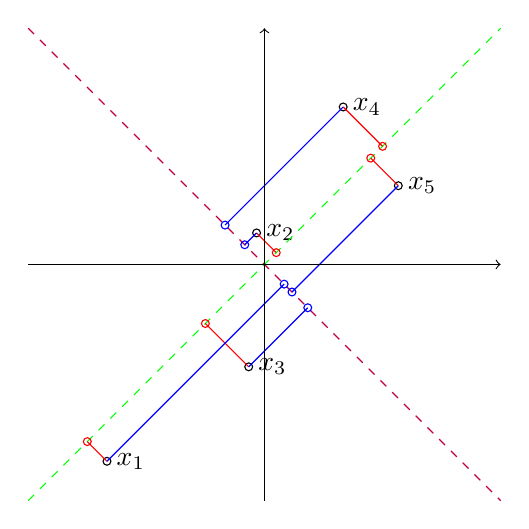
\begin{tikzpicture}
			\coordinate[](origin) at (0,0) ;
			\coordinate[](x1) at (-2,-2.5) ;
			\coordinate[](x2) at (-0.1,0.4) ;
			\coordinate[](x3) at (-0.2,-1.3);
			\coordinate[](x4) at (1,2);
			\coordinate[](x5) at (1.7, 1);
			
			\draw[](x1)circle (0.05) node[xshift=2ex]{$x_1$};
			\draw[](x2)circle (0.05) node[xshift=2ex]{$x_2$};
			\draw[](x3)circle (0.05) node[xshift=2ex]{$x_3$};
			\draw[](x4)circle (0.05) node[xshift=2ex]{$x_4$};
			\draw[](x5)circle (0.05) node[xshift=2ex]{$x_5$};
			
			\draw[dashed, green](-3,-3)--(3,3);
			\draw[red](x1)--(-2.25,-2.25) circle (0.05);
			\draw[red](x2)--(0.15,0.15) circle (0.05);
			\draw[red](x3)--(-0.75,-0.75) circle (0.05);
			\draw[red](x4)--(1.5,1.5) circle (0.05);
			\draw[red](x5)--(1.35,1.35) circle (0.05);
			
			\draw[dashed, purple](-3,3)--(3,-3);
			\draw[blue,thin](x1)--(.25,-.25) circle (0.05);
			\draw[blue,thin](x2)--(-0.25,0.25) circle (0.05);
			\draw[blue,thin](x3)--(0.55,-0.55) circle (0.05);
			\draw[blue,thin](x4)--(-0.5,0.5) circle (0.05);
			\draw[blue,thin](x5)--(0.35, -0.35) circle (0.05);
			
			\draw[->] (-3,0) -- (3,0);
			\draw[->] (0,-3) -- (0,3);
			\end{tikzpicture}
			\caption{Visual of projected variance maximization.}
		\end{figure}
		Clearly the pruple line has lower projected variance than the green line. Intuitively the worst case line would project all points onto the same point, losing all inforamation (variance). The best case would maximize the the variance. Variance of the priojections can then be seen as how much information is retained when projecting.
		\section{Principal Component Analysis(PCA)}
		We've seen the case of a single line, now we could ask ourselves, \textit{Could we perform another projection to reduce the dimension again?}. Let's take a look at the so called "residual", which is the original data point minus the projected data point:
		\begin{equation}
			\label{eq:residual_definition}
			\begin{split}
				 r_i := x_i - (a + bz_i) &= x_i - (x_i)^Tbb\\
				 &=(\ID - bb^T)x_i
			\end{split}
		\end{equation}
		The above result was derived using $x_i^Tbb = bx_i^Tb=bb^Tx_i$. Figure \ref{fig:residual} shows what the redisual looks like, however since there are only $2$ dimensions it's somewhat less clear.
		\begin{figure}[h!]
			\centering
			\begin{tikzpicture}
			\coordinate[](origin) at (0,0) ;
			\coordinate[](x1) at (-2,-2.5) ;
			\coordinate[](x2) at (-0.1,0.4) ;
			\coordinate[](x3) at (-0.2,-1.3);
			\coordinate[](x4) at (1,2);
			\coordinate[](x5) at (1.7, 1);
			
			\draw[](x1)circle (0.05) node[xshift=2ex]{$x_1$};
			\draw[](x2)circle (0.05) node[xshift=2ex]{$x_2$};
			\draw[](x3)circle (0.05) node[xshift=2ex]{$x_3$};
			\draw[](x4)circle (0.05) node[xshift=2ex]{$x_4$};
			\draw[](x5)circle (0.05) node[xshift=2ex]{$x_5$};
			
			\draw[dashed, green](-3,-3)--(3,3);
			\draw[->, red](x1)->(-2.25,-2.25) circle (0.05);
			\draw[->, red](x2)->(0.15,0.15) circle (0.05);
			\draw[->, red](x3)->(-0.75,-0.75) circle (0.05);
			\draw[->, red](x4)->(1.5,1.5) circle (0.05);
			\draw[->, red](x5)->(1.35,1.35) circle (0.05);
			
			\draw[->](origin) -- (0.25,-0.25);
			\draw[->](origin) -- (-0.25,0.25);
			\draw[->](origin) -- (0.55,-0.55);
			\draw[->](origin) -- (-0.5, 0.5);
			\draw[->](origin) -- (0.35,-0.35);
			
			\draw[->] (-3,0) -- (3,0);
			\draw[->] (0,-3) -- (0,3);
			\end{tikzpicture}
			\caption{Visualisation of residuals.}
			\label{fig:residual}
		\end{figure}\\
		\subsection{PCA as an iterative process}
		What if we again try to project the residual to an optimal line, we simply treat the residuals as our new data? Note that then the analasys to do this is axactly the same case as in previous sections. We also need the fact that the mean of the residuals is again centered since:
		\begin{equation}
			\frac{1}{n}\sum_{i=1}^{n}r_i = (\ID - bb^T)\frac{1}{n}\sum_{i=1}^{n}x_i = 0
		\end{equation}
		This means that the analysis can be done exactly the same. Like in previous section, minimizing $\sum_{i-1}^{n}\norm{r_i^Tbb - r_i}^2$ for b will result in having to maximize $b^T(\frac{1}{n}\sum_{i=1}^{n}r_ir_i^T)b = b^T\Sigma_rb$ for b. \\\\
		We could simply find the principal eigenvector of $\Sigma_r $ and do this iteratively, but maybe we could exploit a relationship to make it simpler. So what is the relationship between $\Sigma_r$ and $\Sigma$? We analyse this as follows using (\ref{eq:residual_definition}), the fact that $(\ID - bb^T)$ is idempotent as shown in(\ref{eq:idempot}) and that $\Sigma$ is symmetric:
		\begin{equation}
			\begin{split}
				\frac{1}{n}\sum_{i=1}^{n}r_ir_i^T &= \frac{1}{n}\sum_{i=1}^{n}(\ID - bb^T)x_i((\ID - bb^T)x_i)^T\\
					&= \frac{1}{n}\sum_{i=1}^{n}(\ID - bb^T)x_ix_i^T(\ID - bb^T)^T\\
					&= (\ID - bb^T)(\ID - bb^T)\Sigma^T\\	
					&= \Sigma - b\Sigma b^T\\
					&= \Sigma - \lambda bb^T			
			\end{split}
		\end{equation}
		We can already notice something immediately, $b$ (the eigenvector of $\Sigma$) is now also an eigenvector of $(\Sigma - \lambda bb^T)$:
		\begin{equation}
		(\Sigma - \lambda bb^T)b = \Sigma b - \lambda b = 0\\
		\end{equation}
		The reverse is obviously true an eigenvector of $(\Sigma - \lambda bb^T)$ is also an eigenvector of $\Sigma$, it follows from the previous.
		This $v$ is the principal eigenvector of $(\Sigma - \lambda bb^T)$ (by construction) and the second principle eigenvector of $\Sigma$, by iterating $m$ times we find $d$ pairwise othogonal eigenvectors. Figure \ref{fig:residual} shows visually that using the residuals to find an optimal projection will find maximum projected variance when the line is orthogonal to the green line. Another way to see why they are orthogonal is by noting that $\Sigma$ is positive semi-definite ($\lambda_i > 0$) because it's symmetric so the eigenvectors are orthogonal\footnote{say $x$ and $y$ are eigenvectors with $\lambda_1$ and $\lambda_2$ as eigenvalues of $A$ then $\lambda_1 <x,y> = <Ax,y> = <x,A^Ty> = <x,Ay>=<x,y>\lambda_2$ since $\lambda_1 \neq \lambda_2$ then $<x,y>=0$.}
		\subsection{PCA as a diagonalization problem}
		Recall that $\Sigma$ is symmetric so it may be diagonalized into orthogonal matrices:
		\begin{equation}
		\Sigma = U\Lambda U^T
		\end{equation}
		Where $U=(u_1, u_2, \dots, u_m)$ and $\Lambda = diag(\lambda_1, \dots, \lambda_m)$ note that the eigenvectors are orthogonal so that:
		\begin{equation}
			U^Tu_i = \begin{bmatrix}
			u_1^T\\
			\vdots\\
			u_m^T
			\end{bmatrix}u_i = \begin{bmatrix}
			u_1^Tu_i\\
			\vdots\\
			u_m^Tu_i
			\end{bmatrix} = \begin{bmatrix}
			0\\
			\vdots\\
			u_i^Tu_i = 1\\
			\vdots\\
			0\\
			\end{bmatrix}=e_i
		\end{equation}
		Using this we can clearly see that:
		\begin{equation}
		\begin{split}
			U\Lambda U^T & =\begin{bmatrix}
			u_1 & \dots & u_m\\
			\end{bmatrix}
			\begin{bmatrix}
			\lambda_1 &\dots & 0\\
			\vdots&\cdots&\vdots\\
			0& \dots& \lambda_m\\
			\end{bmatrix}
			\begin{bmatrix}
			u_1 \\ \vdots \\ u_m\\
			\end{bmatrix}		\\
			&=\begin{bmatrix}
			\lambda_1u_1 & \dots & \lambda_mu_m\\
			\end{bmatrix}\begin{bmatrix}
			u_1 \\ \vdots \\ u_m\\
			\end{bmatrix}\\
			&= \Sigma \underbrace{UU^T}_{\ID} = \Sigma
		\end{split}
		\end{equation}
		\subsection{Colclusion: PCA}
		Let's recap what we did to find out what PCA is.\\
		
		 First we want to reduce our data from higher dimension to lower dimension. We first considered a line of the simple form $a+bz$, to attemt to reduce dimension. We concluded that using the euclidean distance the optimal point (minimal distance) on the line was the point such that if we project $x_i$ onto it.\\
		 
		 Second we looked at what the ideal offset $a$ for the euclidean distance given a set of data points $x_i, 1\leq i \leq n$. It of course turned out to be the center of mass $\frac{1}{n}\sum_{i=1}^{n}x_i$. We then decided to shift the entire dataset by substracting the center of mass from every datapoint. This makes analasys way easier.\\
		 
		 Third we looked at the optimal direction $b$ of the line and it turned out that the objective funtion was finding the principal eigenvector of the biased empirical variance $\Sigma = \frac{1}{n}\sum_{i=1}^{n}x_ix_i^T$. Another way of looking at it was maximizing the variance of the projected points $x_i$.\\
		 
		 Fourth we looked at iterative PCA by again projecting the residuals $r_i = x_i - x_i^Tbb$ on another (orthogonal) line. This was again an eigenvector of $\Sigma$, the construction of can be done iteratively. Another way to look at it was as a diagonalization problem of $\Sigma = U\Lambda U^T$.\\
		 
		 Now where is the "reduction" of the data exactly? Well every point can be projected to $d$ principle eigenvectors of $\Sigma$ to give us $U^T x_i = (u_1^Tx_i \dots u_dx_i) = (z_1 \dots z_d)$ this gives us a reduction to the optimal weights for a linear combination of the lower dimensional basis (the $d$ principal eigenvectors). To re-construct the data point we take a linear combination of the $d$ principal eigenvectors. This can be done as $(z_1 \dots z_d)U$. Of course when you pick $d$ to be the dimensionality of the data then there is no reduction but an exact decomposition of the data matrix $X$. So basically:
		 \begin{itemize}
		 	\item Reduction: \begin{equation}
		 	Z = U^T X= \begin{bmatrix}
		 	u_1\\
		 	\vdots\\
		 	u_d\\
		 	\end{bmatrix}
		 	\begin{bmatrix}
		 	x_1&
		 	\dots&
		 	x_n\\
		 	\end{bmatrix} = 
		 	\begin{bmatrix}
		 	x_1^Tu_1 & \dots& x_nu_1\\
		 	\vdots& \cdots & \vdots\\
		 	x_1u_d & \dots & x_nu_d\\
		 	\end{bmatrix} = \begin{bmatrix}
		 	z_{1,1} & \dots& z_{n,1}\\
		 	\vdots& \cdots & \vdots\\
		 	z_{1,d} & \dots & z_{n,d}\\
		 	\end{bmatrix}
		 	\end{equation}
		 	we can clearly see that we reduced the data from $\Real^m$ to $\Real^d$. Only if $d < m$ is there really a reduction and is there truly an approximation when reconstructing!
		 	\item Re-construction:
		 	\begin{equation}
		 	\hat{X} = UZ = \begin{bmatrix} 
		 	\sum_{i=1}^{d}z_{1,i}u_i & \dots & \sum_{i=1}^{d}z_{n,i}u_i \\
		 	\end{bmatrix}
		 	\end{equation}
		 	Here I wrote it out explicitly so it's easy to see that the reduction is just keeping track of weights for the linear combination of the $d$ principal eigenvectors.
		 \end{itemize}
	 \section{Practical PCA: Finding pricipal eigenvector}
	 We've seen a derivation of PCA, one perspective of PCA is iteratively finding pricipal eigenvectors or certain symmetric matrices (empirical biased covariance matrix of the data or residuals). However we "skipped" the part where we actually find the principal eigenvector. One practicle way of finding the principal eigenvector is the power method.
	 \subsection{Power method: practicle principal eigenvector}
	 Assume a symmetric matrix $\Sigma$ and we wish to find $u_1$, the principal eigenvector of $\Sigma$. The algorithm goes as follows:
	 \begin{enumerate}
	 	\item Initialize $v_0$ a random vector. For simplicity we assume that $\langle u_1,v_0\rangle \not 0$ and that the principal eignenvalue is unique i.e. $|\lambda_1| > |\lambda_j|$.
	 	\item Iteratively apply the following operation:
	 \begin{equation}
		 v_{t+1} = \frac{\Sigma v_t}{\norm{\Sigma v_t}}
	 \end{equation}
	 \item It holds that:
	 \begin{equation}
		 \lim_{t\rightarrow\infty} v_t = u_1
	 \end{equation}
	 \item To find the corresponding eignenvalue:
	 \begin{equation}
		 \lambda_1 = \lim_{t\rightarrow\infty} \frac{\norm{\Sigma v_t}}{\norm{v_t}} = \frac{\norm{\Sigma u_1}}{\norm{u_1}} = \frac{\norm{\lambda_1u_1}}{\norm{u_1}} = \lambda_1
	 \end{equation}
	\end{enumerate}
	Why does this algorithm work? We assume $\Sigma$ (as in last section) is p.s.d. and symmetric (true for $XX^T$). In this case the eigenvectors are all orthogonal to each other so they can form a basis for $\Real^m$, this means any $v_0 \in \Real^m$ can be written as a linear combination of eigenvectors
	\begin{equation}
	\label{eq:eigenbasis}
	v_0 = \sum_{i=1}^{m} a_i u_i
	\end{equation}
	how does $v_t$ evolve considering this?
	\begin{equation}
	\label{eq:evolve_power}
	v_{t} = \frac{\Sigma^t v_0}{\norm{\Sigma^t v_0}} = \frac{\sum_{i=1}^{m}a_i\Sigma^t u_i}{\norm{\Sigma^t v_0}}
	\end{equation}
	Note equation (\ref{eq:evolve_power}) was obtained by recursively finding $v_i$ and using (\ref{eq:eigenbasis}). Since $u_i$ are eigenvectors by assumption we can re-write it as follows by pulling out the highest eigenvalue:
	\begin{equation}
	\frac{a_1\lambda_1^tu_1 + \sum_{i=2}^{m}\frac{a_i}{a_1}(\frac{\lambda_i}{\lambda_1})^t u_i}{\norm{\Sigma^t v_0}}
	\end{equation}
	To understand the limit as $t\rightarrow\infty$ we clearly see for the numerator:
	\begin{equation}
	\lim_{t\rightarrow\infty}a_1\lambda_1^tu_1 + \sum_{i=2}^{m}\frac{a_i}{a_1}(\underbrace{\frac{\lambda_i}{\lambda_1}}_{=0})^t u_i = a_1\lambda_1^tu_1
	\end{equation}
	The denomenator can be interpreted in the same way (using $\norm{u_1} = 1$), cancelling the $a_1\lambda_1^t$ resulting in power iteration method converging to $u_1$.
	\section{Practical PCA: choosing amount of eigenvectors}
	How many eigenvectors should we "select" or "keep" and how should we select which ones to keep and not keep. Intuitively from previous section which looked at PCA as a variance maximisation of the projected data, we should keep the $k$ eigenvectors which have the highest eigenvalues. It represents how much information is contained within the eigenvector for specific data.\\
	
	This leaves the question, how many of the top eivenvectors should we keep? This has to be decided in a more empirical way, for example one could gather all eigenvalues and sort them and plot their value against index as follows:
	\begin{figure}[h!]
		\centering
		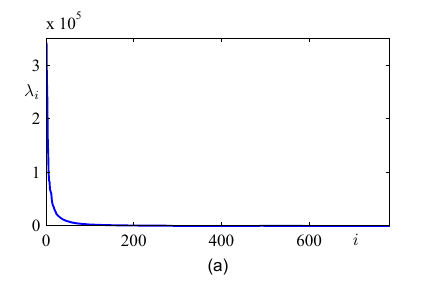
\includegraphics[scale = 0.7]{\figDir/eigenspectrum.PNG}
		\label{fig:eigenspectrum}
		\caption{Sorted eigenvalues plotted against index}
	\end{figure}
	\pagebreak
	In this case it seems like taking the top 50 eigenvectors to represent a reduced dataset would be a good approximation. An engineering rule would be to cut off at "the knee" where the eigenspectrum starts to plateau rapidly.
